% LaTeX Article Template - customizing header and footer
\documentclass{article}

\newtheorem{thm}{Theorem}

% Set left margin - The default is 1 inch, so the following 
% command sets a 1.25-inch left margin.
\setlength{\oddsidemargin}{0.25in}

% Set width of the text - What is left will be the right margin.
% In this case, right margin is 8.5in - 1.25in - 6in = 1.25in.
\setlength{\textwidth}{6in}

% Set top margin - The default is 1 inch, so the following 
% command sets a 0.75-inch top margin.
\setlength{\topmargin}{-0.25in}

% Set height of the header
\setlength{\headheight}{0.3in}

% Set vertical distance between the header and the text
\setlength{\headsep}{0.2in}

% Set height of the text
\setlength{\textheight}{9in}

% Set vertical distance between the text and the
% bottom of footer
\setlength{\footskip}{0.1in}

% Set the beginning of a LaTeX document
\usepackage{multirow}
\usepackage{fullpage}
\usepackage{graphicx}
\usepackage{amsthm}
\usepackage{url}
\usepackage{amssymb}
\usepackage{amssymb}
\usepackage{algpseudocode}
\graphicspath{%
    {converted_graphics/}% inserted by PCTeX
    {/}% inserted by PCTeX
}
%%%%%%%%%%%%%%%%%%%%%%%%%%%%%




\begin{document}\title{Homework $1$\\ Computer Science \\ B351 Spring 2017\\ Prof. M.M. Dalkilic}         % Enter your title between curly braces
\author{Your Name}        % Enter your name between curly braces
\date{\today}          % Enter your date or \today between curly braces
\maketitle


% Redefine "plain" pagestyle
\makeatother     % `@' is restored as a "non-letter" character




% Set to use the "plain" pagestyle
\pagestyle{plain}
All the work herein is mine.
\section*{Introduction}
The aim of this homework is to get you acquianted with problem solving and the steps  (Real World $\rightarrow$ Concept $\rightarrow$ Logic  $\rightarrow$ Implementation).  You will turn-in three files\begin{itemize} \item A *pdf with the written answers called \texttt{h1.pdf} \item A Python script called \texttt{p1.py} for the drone scanning the floor plan \item  A Python script called  \texttt{p2.py} for rock-paper-scissors \end{itemize}.  If you've attempted extra credit, add the comment \#ExtraCredit to the programs and ExtraCredit to the homework near the top so it's visible and obvious.  I am providing this \LaTeX{} document for you to freely use as well. Please enjoy this homework and ask yourself what interests you and then how can you add that interest to it!  Finally, each homework question is worth 100 points.
\newpage
\section*{Homework Questions}
\begin{enumerate}
\item Problem 3.2 in the text.
\item Define {\it Artificial Intelligence} as rational behavior.  What is a problem that AI is {\it not} suited for?
\item Assume you're programming an office security drone who's mission is to move through a floor, checking for any movement.  You've been given the floor plan shown below.  There are two entrances to the floor: \textsf{L, C}.  
\begin{center}
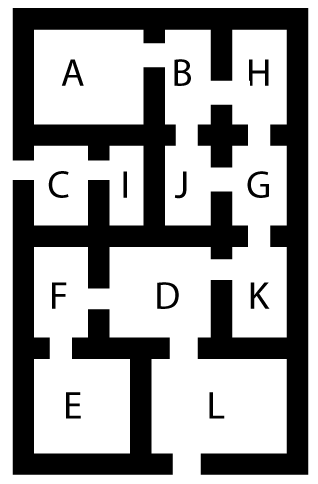
\includegraphics[scale=0.40]{maze55}
\end{center}
\begin{enumerate}
\item Using a graph $ G = (V,E)$, model this plan so that the drone can navigate the floor.  ({\it hint}) You'll need to have an additional vertex that represents the outside--call this vertex \textsf{U}.  $G$ is  an {\it undirected} graph (edges have no direction).  And edge is now either $\{u,v\}$ or $\{(u,v), (v,u)\}$.  This impacts the implementation.    For an adjancency list, you'll have to decide whether to have one edge or both. 
\item Using an adjacency list, model this floor plan.
\item Trace a DFS on $G$ starting at \textsf{U}.
\item The drone takes 4 minutes to scan a room and 2 minutes to move from one room to another.  The drone needs 7 minutes to move from \textsf{L} to \textsf{C} (or {\it vice versa}.  What is the approximate total time it takes for the drone to check the floor?  How would you annotate the graph to reflect this cost? ({\it You're not asked to redo the graph--just explain what you'd do})
\item A single battery for the drone holds about 45 minutes worth of charge.  How many batteries does the drone need to scan the floor?
\item Using Python, create an adjacency list data structure (I used a dictionary which seems reasonable); then using either a Python package or your own implementation, do a DFS from the {\it outside} of the floor, {\it i.e.,} DFS($G$, \textsf{U}).  The DFS should yield a sequence of rooms that the drone would scan.
\item For extra credit, add the cost to the drone and battery life to the search; when the drone has scanned all the rooms, give the percent battery life left. 
\item For extra extra credit, presume the drone starts and ends at \textsf{U}.
\end{enumerate}
\item Rock/Paper/Scissors is a simple game: numbers 0,1,2 denotes each of these items with an outcome that rock {\it beats} scissors, scissors {\it cut} paper, and paper {\it covers} rock; otherwise it's a tie.  Included below (and as file) is a Python script that allows a human to play with a computer. 
\begin{figure}[h]
{\small
\begin{verbatim}
import random as rn

#values of rock, paper, scissors
r,p,s = 0,1,2
#dictionary e.g., rock beats scissors
ws = {r:s, p:r, s:p}

nogames = int(input("Number of games? "))

totgames = 0
compwins = 0
humwins = 0
ties = 0

gamehistory = []

while totgames < nogames:
     human = int(input("r=0,p=1,s=2 "))
     comp = rn.randrange(0,3,1)
     gamehistory.append([human, comp])

     print("Human: {0}, Comp: {1}".format(human, comp))

     if ws[comp] == human:
        compwins += 1
     elif ws[human] == comp:
        humwins += 1
     else:
        ties += 1
     totgames += 1

v = list(map(lambda x: 100*x/totgames, [compwins, humwins, ties]))
print("Stats\ncw% = {0}, hm% = {1}, ties% = {2}".format(*v))
\end{verbatim}}
\end{figure}
\begin{enumerate}
\item Play 5 times of 10 games (it will go quickly) and record the statistics for your wins, $H_1, H_2, \ldots, H_5$.   {\it Expectation} gives us a measure of central tendency (sometimes called the mean).  We can calculate the expectation as
\begin{eqnarray*}
\mathrm{E}[H] &=& \sum_{i=1}^5 H_i/5
\end{eqnarray*}
What is the expecation of a human winning? Are you surpised? Of the computer winning?
\item From \url{python.org} look-up the random function.  How is it picking the numbers 0,1,2?  Does the computer's choice of numbers depend on its previous choice? How about a yours?
\item Remove the human player and add another computer player called Robby.  See if you can find a strategy that has Robby's expected winning greater than the computer.  You are free to employ whatever you'd like so long as it's yours.

\end{enumerate}
\end{enumerate}
\end{document}
